\documentclass[xcolor=table, hyperref={pdfpagelabels=false}]{beamer}
\usepackage{lmodern}
\usepackage[utf8]{inputenc}
\usepackage{tikz}
\usetheme{Frankfurt}
\usepackage{qtree}
\usepackage{subcaption}
\usepackage{float}
\usepackage{graphicx}


\title{Espace conceptuel : de l'homme à la machine}  
\author{Adele Mortier} 
\date{\today} 
\begin{document}

\begin{frame}
\titlepage
\end{frame} 


\begin{frame}
\frametitle{Plan}
\tableofcontents
\end{frame} 
\section{Concepts}
\begin{frame}{Trier nos concepts}
	\begin{figure}
		\centering
		\begin{subfigure}[b]{.45\textwidth}
			\centering
			\includegraphics[width=100px]{./images/casiers.jpg}
			\caption{Des jolis casiers}
		\end{subfigure}\pause
		\begin{subfigure}[b]{.45\textwidth}
			\centering
			\includegraphics[width=100px]{./images/tree.png}
			\caption{Un arbre bien décoré}
		\end{subfigure}
	\end{figure}
\end{frame}
\begin{frame}{Vraiment?}
\begin{figure}
	\centering
	\begin{subfigure}[b]{.45\textwidth}
		\centering
		\includegraphics[height=100px]{./images/apple_watch.jpeg}
		\caption{Bijou? GPS? Coach sportif? Lecteur audio? Téléphone?}
	\end{subfigure}\pause
	\begin{subfigure}[b]{.45\textwidth}
		\centering
		\includegraphics[width=150px]{./images/pianocktail1.jpg}
		\caption{Instrument? Meuble? ``Mixologiste''?}
	\end{subfigure}\pause
	\begin{block}{Conséquences}
		\begin{itemize}
			\item On peut imaginer des concepts qui ne font vraiment partie d'aucun concept.\pause
			\item Du coup, mieux vaut réviser notre idée des concepts!
		\end{itemize}
	\end{block}
\end{figure}
\end{frame}



\begin{frame}{L'approche ``statistique'': \cite{rosch1975,wittgenstein1953}}
\begin{figure}
\centering
\begin{subfigure}[b]{.45\textwidth}
	\centering
	\includegraphics[width=100px]{./images/k_means.png}
	\caption{Clusters et prototypes}
\end{subfigure}
\begin{subfigure}[b]{.45\textwidth}
	\centering
		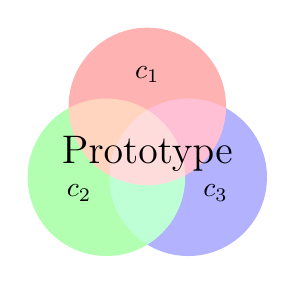
\begin{tikzpicture}[scale=0.50]
		\begin{scope}[blend group = soft light]
		\fill[red!30!white]   ( 90:1.2) circle (2);
		\fill[green!30!white] (210:1.2) circle (2);
		\fill[blue!30!white]  (330:1.2) circle (2);
		\end{scope}
		\node at ( 90:2)    {$c_1$};
		\node at ( 210:2)   {$c_2$};
		\node at ( 330:2)   {$c_3$};
		\node [font=\Large] {Prototype};
		\end{tikzpicture}
		\caption{Prototype maximisant le nombre de traits communs}
\end{subfigure}
\begin{block}{Conséquences}
	\begin{itemize}
		\item \textbf{Étalement} des éléments autour du prototype; \pause
		\item \textbf{Probabilité} d'appartenance à un concept; \pause
		\item \textbf{Faisceau} de traits communs (``air de famille'')
	\end{itemize}
\end{block}
\end{figure}
\end{frame}
\begin{frame}{Lien avec l'apprentissage statistique}
\begin{figure}[H]
	\centering
	\includegraphics[width=200px]{./images/tsne_vgg.png}
	\caption{Projection d'images dans un espace vectoriel}
\end{figure}
\end{frame}
\begin{frame}
\begin{figure}[H]
	\centering
	\includegraphics[width=.90\textwidth]{./images/tsne_vgg_zoom_clusters.png}
	\caption{Apprentissage implicite de sous-catégories}
\end{figure}
\end{frame}
\section{Analogie}
\begin{frame}{Analogie}
\begin{block}{Définition}
	\begin{itemize}
		\item \textit{\textbf{Mapping}} entre ensembles de concepts\pause
		\item L'analogie de \textbf{structure} conserve les relations entre concepts
	\end{itemize}
\end{block}\pause
\begin{figure}[H]
	\begin{subfigure}{.49\textwidth}
		\centering
		\includegraphics[width=.95\textwidth]{./images/kid_analogy.jpeg}
		\caption{L'analogie proportionnelle: un jeu d'enfant}
	\end{subfigure}\pause
	\begin{subfigure}{.49\textwidth}
		\centering
		\includegraphics[width=.65\textwidth]{./images/deep_analogy.png}
		\caption{L'analogie électromécanique: pas trivial!}
	\end{subfigure}
\end{figure}
\end{frame}
\begin{frame}{Au niveau cognitif \cite{holyoak2012}}
	\begin{minipage}{.6\textwidth}
		\begin{block}{Principe}
			\begin{enumerate}
			\item Prise de connaissance du \textbf{problème cible};\pause
			\item Revue des \textbf{analogues pertinents} présents en mémoire;\pause
			\item Choix d'un \textbf{problème source} parmi ces analogues;\pause
			\item \textbf{Mise en relation} entre la source et la cible;\pause
			\item \textbf{Résolution} des parties manquantes (inférence) sur la cible.
		\end{enumerate}
		\end{block}\pause
	\end{minipage}\qquad
	\begin{minipage}{.3\textwidth}
		\begin{figure}[H]
			\centering
			\includegraphics[width=\textwidth]{./images/analogy_cog.png}
			\caption{La résolution de problème comme tâche de \textit{pattern matching}}
		\end{figure}
	\end{minipage}
\end{frame}
\begin{frame}{Lien avec l'apprentissage statistique}
\begin{figure}
	\centering
	\includegraphics[width=280px]{./images/capital_city.png}
	\caption{Concept : Point :: Relation : Vecteur !! \cite{mikolov2013b}}
\end{figure}
\end{frame}
\begin{frame}{Résolution de problèmes}
\begin{figure}[H]
	\centering
	\includegraphics[width=200px]{../images/analogy_vec.png}
	\caption{Résolution vectorielle d'analogie; le point théorique $d'$ est ici \textit{remappé} vers le point $d$, son plus proche voisin qui correspond à une donnée réelle (mot, image etc.)}
\end{figure}
\end{frame}
\section{Conclusion}
\begin{frame}
\begin{block}{Conclusion}\pause
	\begin{itemize}
		\item Ce travail sur l'analogie est lui-même une analogie: entre \textbf{espace conceptuel} et \textbf{espace métrique}.\pause
		\item MAIS: problème de la pauvreté des données.\pause
		\item MAIS: problème des contraintes d'apprentissage.\pause
		\item MAIS: hypothèses très fortes sur les régularités de l'espace.\pause
		\item À VOIR: polysémie, pragmatique, analogies ``profondes''?
	\end{itemize}
\end{block}
\end{frame}
\section*{References}
\begin{frame}[allowframebreaks]
\frametitle{References}
\nocite{*}
\bibliographystyle{apalike}
\bibliography{biblio}
\end{frame}
\end{document}
